\section{Encoders, Decoders, and the Interpreter Analogy}

The first sentence of the abstract ends with ``\ldots that include an encoder and a decoder.''
This sounds like a technical detail, but it is actually describing a very natural idea.

Think about what a human interpreter does at the United Nations.
First, they \emph{listen} to the entire speech in English.
They do not start translating after the first word.
They build up an internal understanding --- the gist, the argument, the nuances.
Then, once they have that understanding, they \emph{produce} the speech in French.

That is the encoder-decoder pattern.

The \textbf{encoder} reads the entire input and produces a representation --- not a translation, not a summary, but a rich internal state that captures what the input \emph{means}.

The \textbf{decoder} takes that representation and generates the output, one piece at a time.

This is worth pausing on, because it is \emph{not} the obvious approach.
The obvious approach to translation would be: read a word, translate it, read the next word, translate it.
That is essentially what Google Translate did in its early days, and it produced gems like translating ``The spirit is willing but the flesh is weak'' into Russian and back as ``The vodka is strong but the meat is rotten.''\footnote{This story is probably apocryphal, but it illustrates the point perfectly.}

The encoder-decoder insight is that you should separate \emph{understanding} from \emph{generating}.
First understand the whole thing.
Then produce the output.

By 2017, this pattern was universal.
Whether you built your system from RNNs or CNNs, you structured it as an encoder followed by a decoder.
It was not a specific architecture --- it was a design principle.

So now we have the full picture of sentence one: in 2017, if you wanted to convert one sequence into another, you used a neural network organized as an encoder-decoder, where the guts of the network were either RNNs (sequential, hard to parallelize) or CNNs (parallelizable, bad at long-range dependencies).

\begin{figure}[htb]
\centering
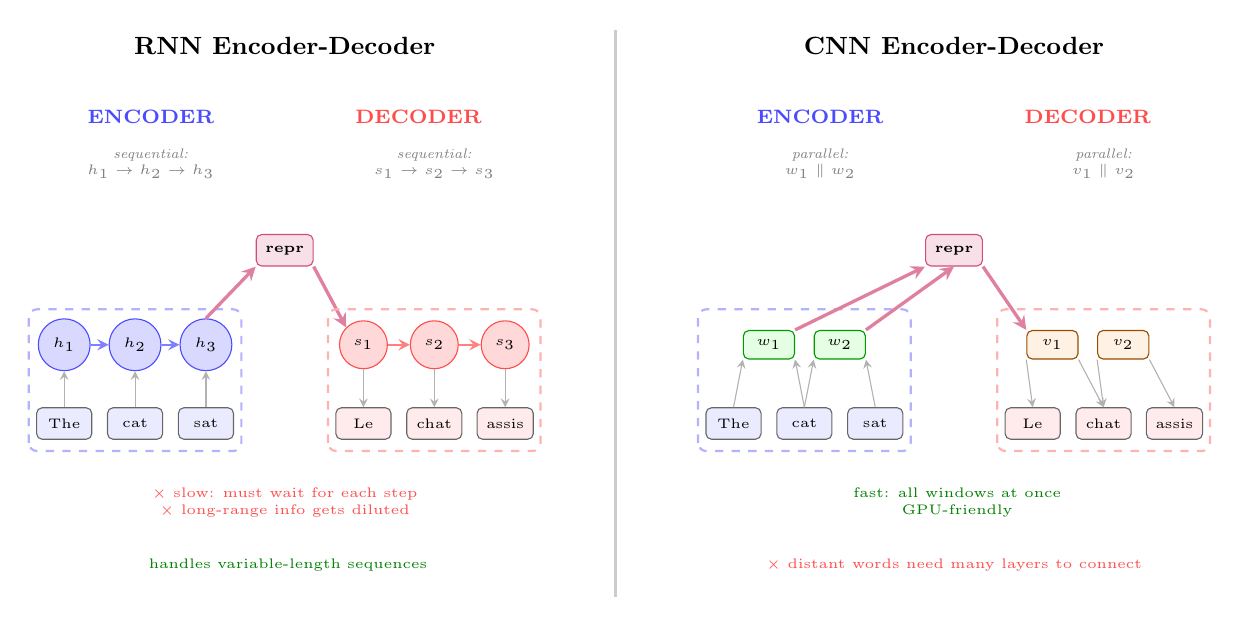
\begin{tikzpicture}[
    >=stealth,
    word/.style={rectangle, draw=black!60, fill=blue!8, rounded corners=2pt,
                 minimum width=0.7cm, minimum height=0.4cm, font=\tiny},
    outword/.style={rectangle, draw=black!60, fill=red!8, rounded corners=2pt,
                    minimum width=0.7cm, minimum height=0.4cm, font=\tiny},
    state/.style={circle, draw=blue!70, fill=blue!15, minimum size=0.45cm, font=\tiny\bfseries},
    dstate/.style={circle, draw=red!70, fill=red!15, minimum size=0.45cm, font=\tiny\bfseries},
    repr/.style={rectangle, draw=purple!70, fill=purple!12, rounded corners=2pt,
                 minimum width=0.7cm, minimum height=0.4cm, font=\tiny\bfseries},
    winbox/.style={rectangle, draw=green!60!black, fill=green!10, rounded corners=2pt,
                   minimum width=0.65cm, minimum height=0.35cm, font=\tiny},
    dwinbox/.style={rectangle, draw=orange!60!black, fill=orange!10, rounded corners=2pt,
                    minimum width=0.65cm, minimum height=0.35cm, font=\tiny},
    arr/.style={->, thick, black!40},
    chain/.style={->, thick, blue!50},
    dchain/.style={->, thick, red!50},
    bigarr/.style={->, very thick, purple!50},
    note/.style={font=\tiny\itshape, text=black!50, align=center},
    feed/.style={->, black!30},
]

  % ===== LEFT COLUMN: RNN Encoder-Decoder =====
  \def\lx{0}

  \node[font=\small\bfseries] at (\lx + 2.8, 4.8) {RNN Encoder-Decoder};

  % Encoder label
  \node[font=\scriptsize\bfseries, text=blue!70] at (\lx + 1.1, 3.9) {ENCODER};

  % Encoder: input words
  \node[word] (re1) at (\lx + 0, 0) {The};
  \node[word] (re2) at (\lx + 0.9, 0) {cat};
  \node[word] (re3) at (\lx + 1.8, 0) {sat};

  % Encoder: hidden states
  \node[state] (rh1) at (\lx + 0, 1) {$h_1$};
  \node[state] (rh2) at (\lx + 0.9, 1) {$h_2$};
  \node[state] (rh3) at (\lx + 1.8, 1) {$h_3$};

  \draw[feed] (re1) -- (rh1);
  \draw[feed] (re2) -- (rh2);
  \draw[feed] (re3) -- (rh3);
  \draw[chain] (rh1) -- (rh2);
  \draw[chain] (rh2) -- (rh3);

  % Encoder brace region
  \draw[blue!30, thick, dashed, rounded corners=3pt]
    (\lx - 0.45, -0.35) rectangle (\lx + 2.25, 1.45);

  % Representation
  \node[repr] (rrep) at (\lx + 2.8, 2.2) {repr};
  \draw[bigarr] (rh3.north) -- (rrep.south west);

  % Decoder label
  \node[font=\scriptsize\bfseries, text=red!70] at (\lx + 4.5, 3.9) {DECODER};

  % Decoder: hidden states
  \node[dstate] (rd1) at (\lx + 3.8, 1) {$s_1$};
  \node[dstate] (rd2) at (\lx + 4.7, 1) {$s_2$};
  \node[dstate] (rd3) at (\lx + 5.6, 1) {$s_3$};

  \draw[bigarr] (rrep.south east) -- (rd1.north west);
  \draw[dchain] (rd1) -- (rd2);
  \draw[dchain] (rd2) -- (rd3);

  % Decoder: output words
  \node[outword] (ro1) at (\lx + 3.8, 0) {Le};
  \node[outword] (ro2) at (\lx + 4.7, 0) {chat};
  \node[outword] (ro3) at (\lx + 5.6, 0) {assis};

  \draw[feed] (rd1) -- (ro1);
  \draw[feed] (rd2) -- (ro2);
  \draw[feed] (rd3) -- (ro3);

  % Decoder brace region
  \draw[red!30, thick, dashed, rounded corners=3pt]
    (\lx + 3.35, -0.35) rectangle (\lx + 6.05, 1.45);

  % Sequential annotation
  \node[note] at (\lx + 1.1, 3.3) {sequential:\\$h_1 \to h_2 \to h_3$};
  \node[note] at (\lx + 4.7, 3.3) {sequential:\\$s_1 \to s_2 \to s_3$};

  % Tradeoff
  \node[font=\tiny, text=red!70, align=center] at (\lx + 2.8, -1.0)
    {$\times$ slow: must wait for each step\\$\times$ long-range info gets diluted};
  \node[font=\tiny, text=green!50!black, align=center] at (\lx + 2.8, -1.8)
    {$\checkmark$ handles variable-length sequences};

  % ===== RIGHT COLUMN: CNN Encoder-Decoder =====
  \def\rx{8.5}

  \node[font=\small\bfseries] at (\rx + 2.8, 4.8) {CNN Encoder-Decoder};

  % Encoder label
  \node[font=\scriptsize\bfseries, text=blue!70] at (\rx + 1.1, 3.9) {ENCODER};

  % Encoder: input words
  \node[word] (ce1) at (\rx + 0, 0) {The};
  \node[word] (ce2) at (\rx + 0.9, 0) {cat};
  \node[word] (ce3) at (\rx + 1.8, 0) {sat};

  % Encoder: conv summaries (parallel)
  \node[winbox] (cw1) at (\rx + 0.45, 1) {$w_1$};
  \node[winbox] (cw2) at (\rx + 1.35, 1) {$w_2$};

  \draw[feed] (ce1.north) -- (cw1.south west);
  \draw[feed] (ce2.north) -- (cw1.south east);
  \draw[feed] (ce2.north) -- (cw2.south west);
  \draw[feed] (ce3.north) -- (cw2.south east);

  % Encoder brace region
  \draw[blue!30, thick, dashed, rounded corners=3pt]
    (\rx - 0.45, -0.35) rectangle (\rx + 2.25, 1.45);

  % Representation
  \node[repr] (crep) at (\rx + 2.8, 2.2) {repr};
  \draw[bigarr] (cw1.north east) -- (crep.south west);
  \draw[bigarr] (cw2.north east) -- (crep.south);

  % Decoder label
  \node[font=\scriptsize\bfseries, text=red!70] at (\rx + 4.5, 3.9) {DECODER};

  % Decoder: conv summaries (parallel)
  \node[dwinbox] (dw1) at (\rx + 4.05, 1) {$v_1$};
  \node[dwinbox] (dw2) at (\rx + 4.95, 1) {$v_2$};

  \draw[bigarr] (crep.south east) -- (dw1.north west);

  % Decoder: output words
  \node[outword] (co1) at (\rx + 3.8, 0) {Le};
  \node[outword] (co2) at (\rx + 4.7, 0) {chat};
  \node[outword] (co3) at (\rx + 5.6, 0) {assis};

  \draw[feed] (dw1.south west) -- (co1.north);
  \draw[feed] (dw1.south east) -- (co2.north);
  \draw[feed] (dw2.south west) -- (co2.north);
  \draw[feed] (dw2.south east) -- (co3.north);

  % Decoder brace region
  \draw[red!30, thick, dashed, rounded corners=3pt]
    (\rx + 3.35, -0.35) rectangle (\rx + 6.05, 1.45);

  % Parallel annotation
  \node[note] at (\rx + 1.1, 3.3) {parallel:\\$w_1 \parallel w_2$};
  \node[note] at (\rx + 4.7, 3.3) {parallel:\\$v_1 \parallel v_2$};

  % Tradeoff
  \node[font=\tiny, text=green!50!black, align=center] at (\rx + 2.8, -1.0)
    {$\checkmark$ fast: all windows at once\\$\checkmark$ GPU-friendly};
  \node[font=\tiny, text=red!70, align=center] at (\rx + 2.8, -1.8)
    {$\times$ distant words need many layers to connect};

  % Dividing line
  \draw[black!20, thick] (7, -2.2) -- (7, 5.0);

\end{tikzpicture}
\caption{The two encoder-decoder approaches of 2017, side by side. \textbf{Left:} RNN-based --- the encoder and decoder each process words sequentially, passing hidden states along a chain. Fast at handling variable lengths, but slow and prone to forgetting.
\textbf{Right:} CNN-based --- both sides process local windows in parallel. Fast to train, but distant words only interact after stacking many layers.}
\end{figure}

And everyone was looking for something better.
